\documentclass{standalone}
\usepackage{tikz}
\usetikzlibrary{patterns, positioning}
\usepackage[sfdefault]{ClearSans} %% option 'sfdefault' activates Clear Sans as the default text font
\usepackage[T1]{fontenc}

\begin{document}
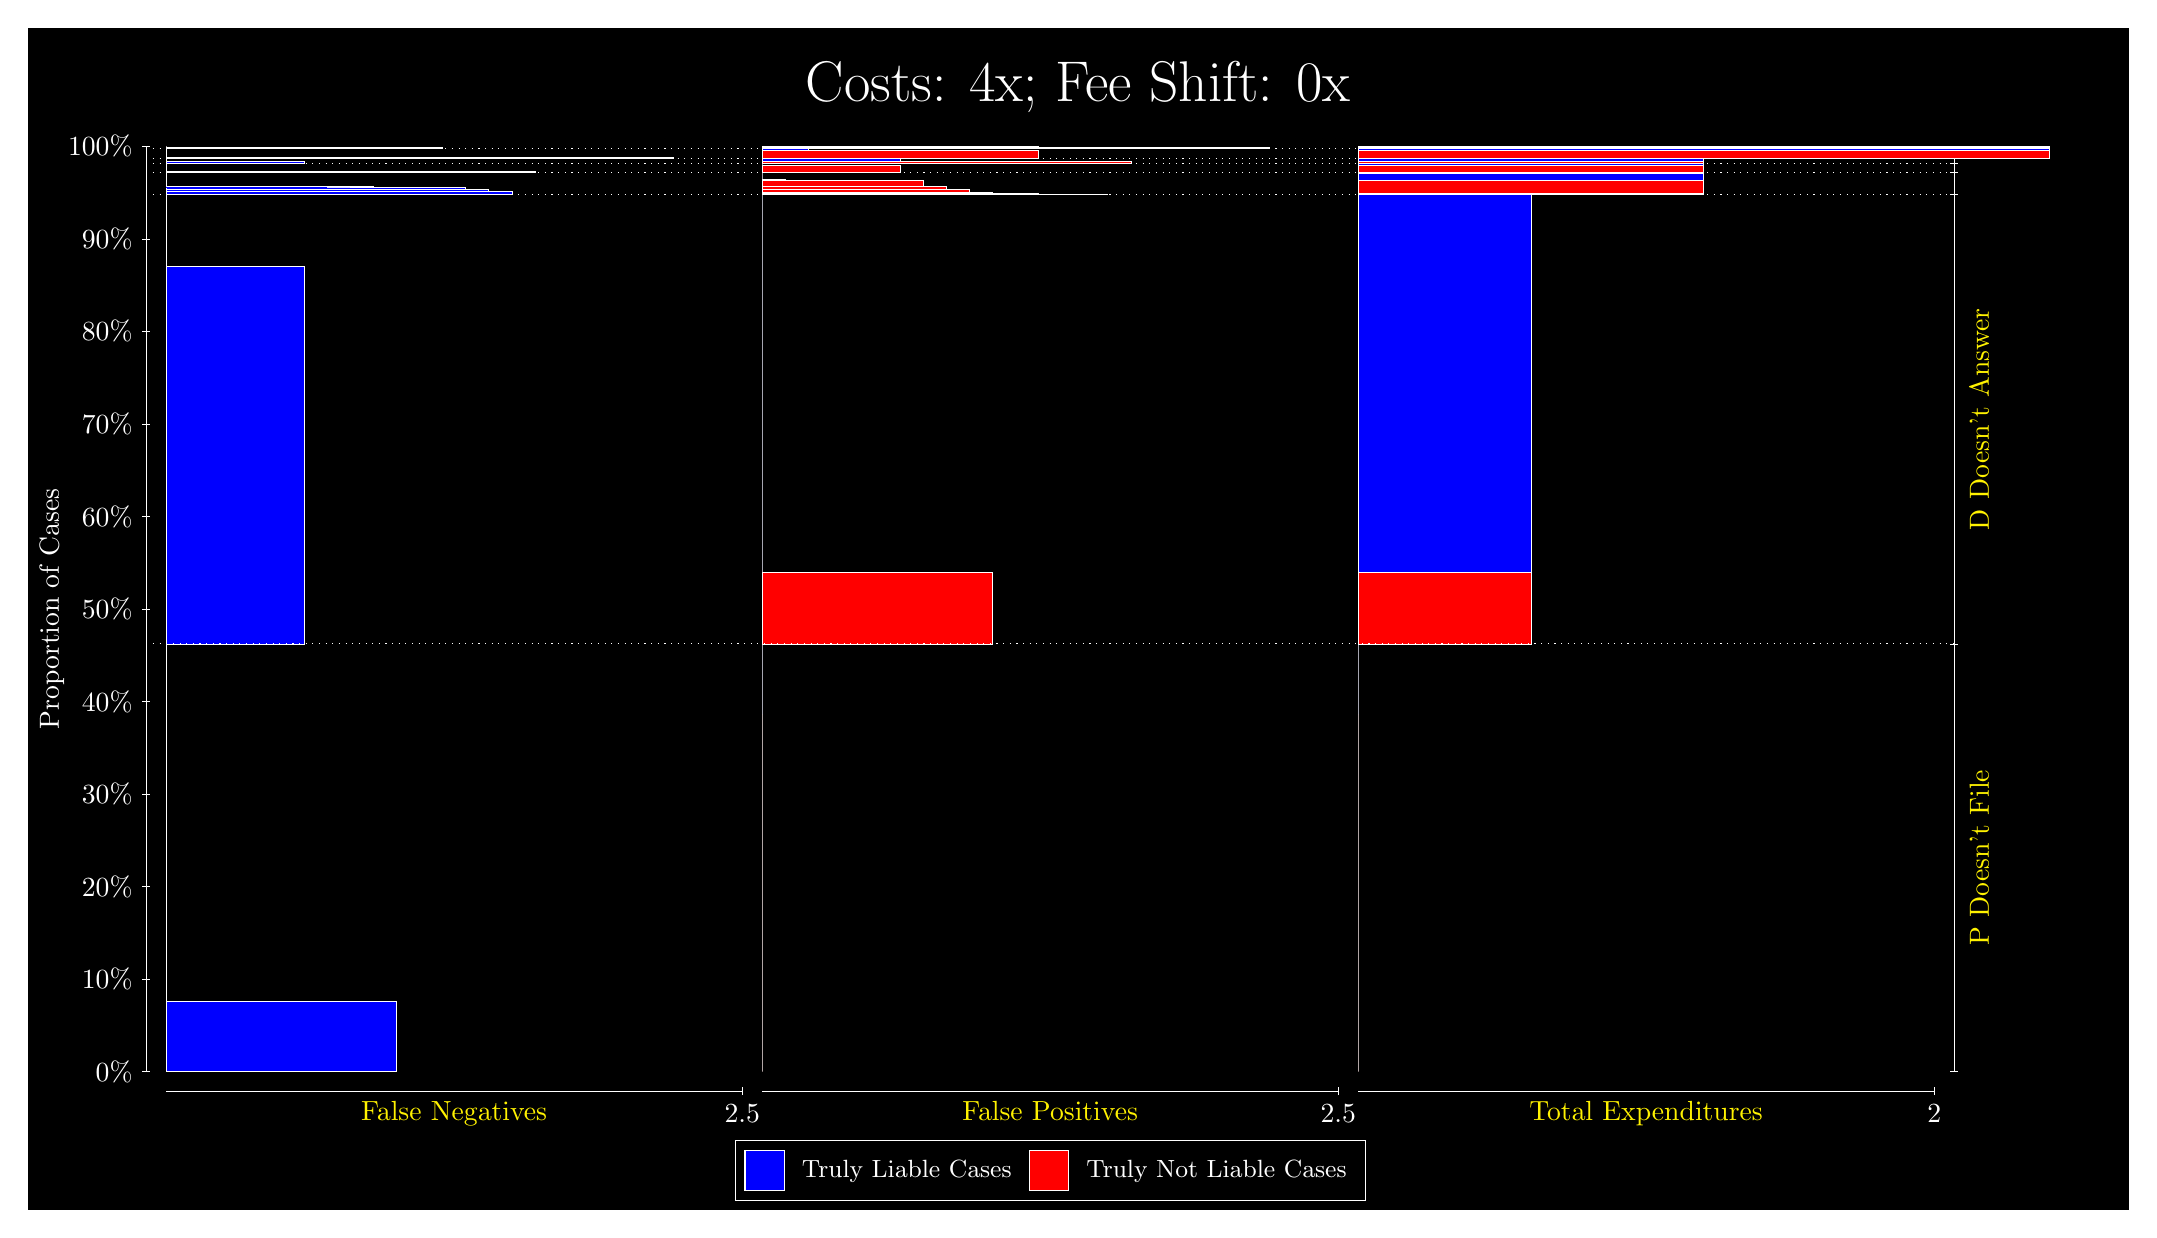
\begin{tikzpicture}
\draw[fill=black] (0,0) rectangle (26.667,15);
\draw[text=white] (0,13.5) rectangle (26.667,15) node[midway] {\huge Costs: 4x; Fee Shift: 0x};
\draw[white, very thin] (1.5,1.75) -- (1.5,13.5);
\node[rotate=90, text=white, anchor=center] at (0.3, 7.625) {Proportion of Cases};
\draw[white, very thin] (1.45,1.75) -- (1.55,1.75);
\node[text=white, anchor=east] at (1.45, 1.75) {0\%};
\draw[white, very thin] (1.45,2.925) -- (1.55,2.925);
\node[text=white, anchor=east] at (1.45, 2.925) {10\%};
\draw[white, very thin] (1.45,4.1) -- (1.55,4.1);
\node[text=white, anchor=east] at (1.45, 4.1) {20\%};
\draw[white, very thin] (1.45,5.275) -- (1.55,5.275);
\node[text=white, anchor=east] at (1.45, 5.275) {30\%};
\draw[white, very thin] (1.45,6.45) -- (1.55,6.45);
\node[text=white, anchor=east] at (1.45, 6.45) {40\%};
\draw[white, very thin] (1.45,7.625) -- (1.55,7.625);
\node[text=white, anchor=east] at (1.45, 7.625) {50\%};
\draw[white, very thin] (1.45,8.8) -- (1.55,8.8);
\node[text=white, anchor=east] at (1.45, 8.8) {60\%};
\draw[white, very thin] (1.45,9.975) -- (1.55,9.975);
\node[text=white, anchor=east] at (1.45, 9.975) {70\%};
\draw[white, very thin] (1.45,11.15) -- (1.55,11.15);
\node[text=white, anchor=east] at (1.45, 11.15) {80\%};
\draw[white, very thin] (1.45,12.325) -- (1.55,12.325);
\node[text=white, anchor=east] at (1.45, 12.325) {90\%};
\draw[white, very thin] (1.45,13.5) -- (1.55,13.5);
\node[text=white, anchor=east] at (1.45, 13.5) {100\%};

\draw[white, very thin] (24.457,1.75) -- (24.457,13.5);
\draw[white, very thin] (24.407,1.75) -- (24.507,1.75);
\node[anchor=west] at (24.407, 1.75) {};
\draw[white, very thin] (24.407,7.1819) -- (24.507,7.1819);
\node[anchor=west] at (24.407, 7.1819) {};
\draw[white, very thin] (24.407,12.888) -- (24.507,12.888);
\node[anchor=west] at (24.407, 12.888) {};
\draw[white, very thin] (24.407,13.169) -- (24.507,13.169);
\node[anchor=west] at (24.407, 13.169) {};
\draw[white, very thin] (24.407,13.282) -- (24.507,13.282);
\node[anchor=west] at (24.407, 13.282) {};
\draw[white, very thin] (24.407,13.343) -- (24.507,13.343);
\node[anchor=west] at (24.407, 13.343) {};
\draw[white, very thin] (24.407,13.475) -- (24.507,13.475);
\node[anchor=west] at (24.407, 13.475) {};
\draw[white, very thin] (24.407,13.5) -- (24.507,13.5);
\node[anchor=west] at (24.407, 13.5) {};

\draw[white, very thin, fill=blue] (1.75,1.75) rectangle (4.6775,2.6428);
\draw[white, very thin, fill=red] (1.75,2.6428) rectangle (1.75,7.1819);
\draw[white, very thin, fill=blue] (1.75,7.1819) rectangle (3.5065,11.976);
\draw[white, very thin, fill=red] (1.75,11.976) rectangle (1.75,12.888);
\draw[white, very thin, fill=blue] (1.75,12.888) rectangle (6.1413,12.933);
\draw[white, very thin, fill=blue] (1.75,12.933) rectangle (5.8486,12.955);
\draw[white, very thin, fill=blue] (1.75,12.955) rectangle (5.5558,12.974);
\draw[white, very thin, fill=blue] (1.75,12.974) rectangle (5.2631,12.979);
\draw[white, very thin, fill=blue] (1.75,12.979) rectangle (4.9703,12.984);
\draw[white, very thin, fill=blue] (1.75,12.984) rectangle (4.6775,12.986);
\draw[white, very thin, fill=blue] (1.75,12.986) rectangle (4.3848,12.988);
\draw[white, very thin, fill=blue] (1.75,12.988) rectangle (4.092,12.988);
\draw[white, very thin, fill=blue] (1.75,12.988) rectangle (3.7993,12.989);
\draw[white, very thin, fill=red] (1.75,12.989) rectangle (1.75,13.169);
\draw[white, very thin, fill=blue] (1.75,13.169) rectangle (6.4341,13.189);
\draw[white, very thin, fill=red] (1.75,13.189) rectangle (1.75,13.282);
\draw[white, very thin, fill=blue] (1.75,13.282) rectangle (3.5065,13.314);
\draw[white, very thin, fill=red] (1.75,13.314) rectangle (1.75,13.343);
\draw[white, very thin, fill=blue] (1.75,13.343) rectangle (8.1906,13.365);
\draw[white, very thin, fill=red] (1.75,13.365) rectangle (1.75,13.475);
\draw[white, very thin, fill=blue] (1.75,13.475) rectangle (5.2631,13.489);
\draw[white, very thin, fill=red] (1.75,13.489) rectangle (1.75,13.5);
\draw[white, very thin, fill=red] (9.3189,1.75) rectangle (9.3189,6.2891);
\draw[white, very thin, fill=blue] (9.3189,6.2891) rectangle (9.3189,7.1819);
\draw[white, very thin, fill=red] (9.3189,7.1819) rectangle (12.246,8.094);
\draw[white, very thin, fill=blue] (9.3189,8.094) rectangle (9.3189,12.888);
\draw[white, very thin, fill=red] (9.3189,12.888) rectangle (13.71,12.89);
\draw[white, very thin, fill=red] (9.3189,12.89) rectangle (13.417,12.891);
\draw[white, very thin, fill=red] (9.3189,12.891) rectangle (13.125,12.894);
\draw[white, very thin, fill=red] (9.3189,12.894) rectangle (12.832,12.898);
\draw[white, very thin, fill=red] (9.3189,12.898) rectangle (12.539,12.906);
\draw[white, very thin, fill=red] (9.3189,12.906) rectangle (12.246,12.912);
\draw[white, very thin, fill=red] (9.3189,12.912) rectangle (11.954,12.952);
\draw[white, very thin, fill=red] (9.3189,12.952) rectangle (11.661,12.995);
\draw[white, very thin, fill=red] (9.3189,12.995) rectangle (11.368,13.068);
\draw[white, very thin, fill=blue] (9.3189,13.068) rectangle (10.783,13.069);
\draw[white, very thin, fill=blue] (9.3189,13.069) rectangle (10.49,13.07);
\draw[white, very thin, fill=blue] (9.3189,13.07) rectangle (10.197,13.071);
\draw[white, very thin, fill=blue] (9.3189,13.071) rectangle (9.9044,13.074);
\draw[white, very thin, fill=blue] (9.3189,13.074) rectangle (9.6116,13.079);
\draw[white, very thin, fill=blue] (9.3189,13.079) rectangle (9.3189,13.169);
\draw[white, very thin, fill=red] (9.3189,13.169) rectangle (11.075,13.263);
\draw[white, very thin, fill=blue] (9.3189,13.263) rectangle (9.3189,13.282);
\draw[white, very thin, fill=red] (9.3189,13.282) rectangle (14.003,13.312);
\draw[white, very thin, fill=blue] (9.3189,13.312) rectangle (11.075,13.343);
\draw[white, very thin, fill=red] (9.3189,13.343) rectangle (12.832,13.453);
\draw[white, very thin, fill=blue] (9.3189,13.453) rectangle (9.9044,13.475);
\draw[white, very thin, fill=red] (9.3189,13.475) rectangle (15.759,13.486);
\draw[white, very thin, fill=blue] (9.3189,13.486) rectangle (12.832,13.5);
\draw[white, very thin, fill=red] (16.888,1.75) rectangle (16.888,6.2891);
\draw[white, very thin, fill=blue] (16.888,6.2891) rectangle (16.888,7.1819);
\draw[white, very thin, fill=red] (16.888,7.1819) rectangle (19.083,8.094);
\draw[white, very thin, fill=blue] (16.888,8.094) rectangle (19.083,12.888);
\draw[white, very thin, fill=red] (16.888,12.888) rectangle (21.279,12.896);
\draw[white, very thin, fill=blue] (16.888,12.896) rectangle (21.279,12.901);
\draw[white, very thin, fill=red] (16.888,12.901) rectangle (21.279,13.07);
\draw[white, very thin, fill=blue] (16.888,13.07) rectangle (21.279,13.164);
\draw[white, very thin, fill=red] (16.888,13.164) rectangle (21.279,13.168);
\draw[white, very thin, fill=blue] (16.888,13.168) rectangle (21.279,13.169);
\draw[white, very thin, fill=red] (16.888,13.169) rectangle (21.279,13.263);
\draw[white, very thin, fill=blue] (16.888,13.263) rectangle (21.279,13.282);
\draw[white, very thin, fill=red] (16.888,13.282) rectangle (21.279,13.312);
\draw[white, very thin, fill=blue] (16.888,13.312) rectangle (21.279,13.343);
\draw[white, very thin, fill=red] (16.888,13.343) rectangle (25.67,13.453);
\draw[white, very thin, fill=blue] (16.888,13.453) rectangle (25.67,13.475);
\draw[white, very thin, fill=red] (16.888,13.475) rectangle (25.67,13.486);
\draw[white, very thin, fill=blue] (16.888,13.486) rectangle (25.67,13.5);
\draw[white, dotted] (1.5,7.1819) -- (24.457,7.1819);
\draw[white, dotted] (1.5,12.888) -- (24.457,12.888);
\draw[white, dotted] (1.5,13.169) -- (24.457,13.169);
\draw[white, dotted] (1.5,13.282) -- (24.457,13.282);
\draw[white, dotted] (1.5,13.343) -- (24.457,13.343);
\draw[white, dotted] (1.5,13.475) -- (24.457,13.475);
\draw[white, very thin] (1.75,1.5) -- (9.0689,1.5);
\node[text=yellow, anchor=north] at (5.4094, 1.5) {False Negatives};
\draw[white, very thin] (9.0689,1.45) -- (9.0689,1.55);
\node[text=white, anchor=north] at (9.0689, 1.45) {2.5};

\draw[white, very thin] (9.3189,1.5) -- (16.638,1.5);
\node[text=yellow, anchor=north] at (12.978, 1.5) {False Positives};
\draw[white, very thin] (16.638,1.45) -- (16.638,1.55);
\node[text=white, anchor=north] at (16.638, 1.45) {2.5};

\draw[white, very thin] (16.888,1.5) -- (24.207,1.5);
\node[text=yellow, anchor=north] at (20.547, 1.5) {Total Expenditures};
\draw[white, very thin] (24.207,1.45) -- (24.207,1.55);
\node[text=white, anchor=north] at (24.207, 1.45) {2};

\node[text=yellow, centered, rotate=90] at (24.777, 4.4659) {P Doesn't File};
\node[text=yellow, centered, rotate=90] at (24.777, 10.035) {D Doesn't Answer};






\draw (12.978300999999998,1.5) node[draw=none] (baseCoordinate) {};
\begin{scope}[align=center]
        \matrix[scale=0.5, draw=white, below=0.5cm of baseCoordinate, nodes={draw}, column sep=0.1cm]{
            \node[rectangle, draw, minimum width=0.5cm, minimum height=0.5cm, fill=blue] {}; &
            \node[draw=none, font=\small, text=white] (B) {Truly Liable Cases}; &
            \node[rectangle, draw, minimum width=0.5cm, minimum height=0.5cm, fill=red] {}; &
            \node[draw=none, font=\small, text=white] (B) {Truly Not Liable Cases}; \\
            };
\end{scope}

\end{tikzpicture}
\end{document}